%
% File ACL2016.tex
%

\documentclass[11pt]{article}
\usepackage{acl2016}
\usepackage{times}
\usepackage{latexsym}
\usepackage{graphicx}
\usepackage{grffile}
\usepackage{hyperref}
\usepackage{tabularx}

%\aclfinalcopy % Uncomment this line for the final submission
%\def\aclpaperid{***} %  Enter the acl Paper ID here

% To expand the titlebox for more authors, uncomment
% below and set accordingly.
% \addtolength\titlebox{.5in}    

\newcommand\BibTeX{B{\sc ib}\TeX}

\title{A better way to detect sarcasm on Twitter? \#yeahright \#notyet}

% Author information can be set in various styles:
% For several authors from the same institution:
% \author{Author 1 \and ... \and Author n \\
%         Address line \\ ... \\ Address line}
% if the names do not fit well on one line use
%         Author 1 \\ {\bf Author 2} \\ ... \\ {\bf Author n} \\
% For authors from different institutions:
% \author{Author 1 \\ Address line \\  ... \\ Address line
%         \And  ... \And
%         Author n \\ Address line \\ ... \\ Address line}
% To start a seperate ``row'' of authors use \AND, as in
% \author{Author 1 \\ Address line \\  ... \\ Address line
%         \AND
%         Author 2 \\ Address line \\ ... \\ Address line \And
%         Author 3 \\ Address line \\ ... \\ Address line}
% If the title and author information does not fit in the area allocated,
% place \setlength\titlebox{<new height>} right after
% at the top, where <new height> can be something larger than 2.25in
\author{Author 1\\
	    XYZ Company\\
	    111 Anywhere Street\\
	    Mytown, NY 10000, USA\\
	    {\tt author1@xyz.org}
	  \And
	Author 2\\
  	ABC University\\
  	900 Main Street\\
  	Ourcity, PQ, Canada A1A 1T2\\
  {\tt author2@abc.ca}}

\date{}

\begin{document}

\maketitle

\begin{abstract}
Sarcasm adds noise to emotion detection and sentiment analysis and has been shown to be a pretty difficult task in general. This project proposes to study the detection of sarcasm in greater detail making use of Twitter data that are annotated with hashtags indicating sarcasm. We first aim to replicate \cite{riloff2013sarcasm}, and then compare it with alternative choices of sarcasm marking hashtags, mainly \#not and \#yeahright, in the bootstrapping data. We observe that the baseline SVM gets an F1-score of 0.33 with a precision and recall of 0.36 and 0.30 respectively on labeling sarcastic tweets as sarcastic, whereas the lexicons derived from the \#sarc dataset and the \#yeahright et al. dataset result in a very small F1-score of not more than 0.05. These results are pending further investigation. On the brighter side, on occasion we do manage to get better precision. Recall, however, remains poor. The lexicons returned by our dataset+algorithm is quite different from the original lexicon in \cite{riloff2013sarcasm}. Recall as measured by the number of recovered terms from the original work is itself poor at this moment. Also, the \#sarc dataset currently beats the \#yeahright dataset in terms of performance. 
\end{abstract}

%2.	What research issue are you investigating? What problem are you trying to solve? Be specific.
\section{Introduction}

This project begins with trying to replicate the work in \cite{riloff2013sarcasm}. Looking at the results of the bootstrapped lexicon in isolation, we note that the best recall they achieved was 29\%. i.e. 71\% of relevant tweets were not classified as sarcastic. Even when the best performing system that combined their Bootstrapped lexicon with the SVM classifier is used for comparison, their recall was 44\%. Once again, 50\% of the relevant tweets were not captured. The authors note that their aim is to identify sarcasm that is self-contained in one tweet and does not depend on prior conversational context. Also, they manually annotated sarcastic tweets and only those tweets that were found sarcastic by humans - that presumably don't require any background knowledge such as context or speaker - were used for measuring precision and recall. Given these statistics, it is safe to say that there are at least 50\% of (human) identifiably context-isolated sarcastic tweets that are not captured by the pattern `Contrast between a Positive Sentiment and Negative Situation". This means there is a great scope for improvement in identifying sarcastic tweets.

We first hypothesize that there might be other patterns like `Contrast between a Positive Sentiment and Negative Situation" that will capture a large proportion of sarcastic tweets. One such pattern that could be a starting point is one that Shereen pointed out: `if...then..." statements, e.g., `if stupidity was a crime then i know a few who deserve imprisonment". This example immediately makes it necessary to have a definition of sarcasm that we can work with. If you look at the example with an `intended meaning contrary to the literal" definition of sarcasm, it might not be classified as sarcasm. However, if you look at the broader class that is stated in \cite{riloff2013sarcasm} - sarcasm is generally characterized as ironic or satirical wit that is intended to insult, mock, or amuse - then it is clear that the aforementioned example is valid. We use the latter, broader definition of sarcasm. It is also apparent from the examples in \cite{riloff2013sarcasm} that their work will only be reproducible with the narrow definition of sarcasm. Once again, this shows scope for improvement in identifying sarcastic tweets. It might be fruitful to ask, what are the other characteristics that define sarcasm? And then ask, what pattern could such a definition imply?

With the general goal being improving the results with \cite{riloff2013sarcasm} as the work to build off of, there are multiple approaches we have in mind. One that is already stated above is looking at complementary patterns. The other explores the hypothesis that the set of positive and negative situations that were arrived at by the bootstrapping algorithm were not optimal. Two reasons are speculated for this suboptimality - a) a suboptimal choice of hashtag (\#sarcasm), b) a suboptimal choice of the seed word (love). It might be instructive to see if results turn out differently when these choices are changed.

We also intend to build upon the following finding from \cite{bamman2015contextualized} "Users are more likely to tag their message with the explicit hashtag \#sarcasm when they are less familiar with their audience". We would like to look for sarcasm patterns in Twitter handles dedicated to sarcastic tweets (\@sarcastweet, for example) for alternate means of sarcasm annotation, since we would also like to look at tweets that are not explicitly marked \#sarcastic, but we know to be sarcastic anyway, just to see if there is a difference between when people find it necessary to annotate sarcasm and when it is obvious.


%8.	What is the current state of the art for this problem? Cite papers. You should be able to cite at least a couple related papers. \section{State of the art}
\section{Related work}

Previous work in sarcasm detection on Twitter states that context is very important. \cite{rajadesingan2015sarcasm} modeled the relationship between a tweet and an author’s past tweet and achieved an accuracy of 83.46\%, while \cite{bamman2015contextualized} also incorporate the addressee of the tweet, and the tweet that it is responding to and achieve a very high accuracy of 84.9\%.  However, without Precision/Recall measures, these results seems incomplete. Also, unlike these papers, we look at strictly self-contained sarcastic tweets that a human who did not know the contextual tweets would still be able to identify as sarcasm.

\cite{ghosh2015semeval} put together a task of sentiment analysis of figurative tweets which included tweets with the hashtag \#sarcasm and \#irony, with 75\% of the training data and 50\% of the test data being this category of tweets. The team that achieved the best results for sarcasm and irony in this task \cite{xu2015llt} makes use of a feature called PolarityShiftWin that is based on the "contrast netween pos and neg" by \cite{riloff2013sarcasm}.

\cite{burgers2012verbal} compares six written genres for ironic utterances for the usage of irony factors and irony markers. Twitter or microblogging, however, are not part of any of the genres.

The SASI system \cite{davidov2010semi} uses a number of features obtained by semisupervised pattern acquisition for identifying sarcasm in Amazon product reviews as well as tweets.

A more detailed review of past work in Sarcasm/Irony detection is available in \cite{tungthamthiti2015sentiment} and \cite{xu2015llt}.
 
 
%\section{Neglected ideas} 
%Can you use the connotation frames paper for sarcasm detection? (I don't think so, because it takes words pretty literally)

 
%3.	What data will you use? Please describe how much data you have, where its from, how it will be annotated or not, etc.
\section{Dataset(s)}

Two datasets were used. Shereen shared a dataset of sarcastic and non-sarcastic tweets in her possession. All of the sarcastic tweets in this dataset, of which there are approximately 80K, were collected using the \#sarc hashtag. There are close to 80K sarcastic tweets. We call this DatasetSarc. Results of bootstrapping using this dataset are compared with results of bootstrapping using a dataset using tweets marked by the hashtags \#irony, \#jk, \#justkidding, \#lol, \#not, \#sarcasm, \#sarcastic, \#sarcastictweet, \#yaright, \#yeahright, \#yearight. These tweets are also approximately 80K in number. This dataset of sarcasm tweets is hereafter called DatasetYeahright. These tweets were downloaded using the Twitter search API.

We have close to 2M tweets that do not contain any sarcasm denoting hashtags (courtesy Shereen). Since the split of sarc:not\_sarc in the \cite{riloff2013sarcasm} paper was 20:80, we randomly chooose 320K tweets out of the 2M for use in bootstrapping. Future work may feature a comparison of results when a different 320K subset is chosen.

%Using the script that the organizers of the SemEval 2015 Task 11 made available, I was able to download about 1000 tweets that were their (annotation) trial data and 8000 tweets that were training data.  We might also have Riloff's gold standard data, which would be very useful for replicating their experiments and looking for patterns that were not captured by their algorithm. Similarly, I want to download more tweets from sarcasm-specific Twitter handles such as @sarcastweet.

While Twitter has the advantage of self-annotation, it might be worthwhile to do a Mechanical Turk task to check how many tweets are identifiable as sarcastic by humans without the hashtag annotation. This may aid in the detection of tweets that do not have self-contained/evident sarcasm. (Perhaps it might be a notable side project to detect tweets that are labeled sarcastic, but cannot be identified as being sarcastic?). For this report, we rely on the availability of Tweets already classified by humans as sarcastic, from the gold standard of \cite{riloff2013sarcasm}.

%9.	Provide samples/examples or exploratory work.
\section{Sample exploratory work}

Alarmingly, 3972 distinct hashtags were used in the 8000 training data tweets of SemEval Task 11. The top ten hashtags are (\#not, 3626), (\#sarcasm, 2108), (\#irony, 1449), (\#yeahright, 55), (\#lol, 34), (\#sarcastictweet, 33), (\#funny, 24), (\#fun, 22), (\#i, 17), (\#im, 17). Clearly, \#not is a better indicator of sarcasm (in the sense of more frequent) than \#sarcasm is, and perhaps running Riloff's bootstrapping algorithm with \#not as the seed might fetch a more diverse range of patterns.

\#justkidding/\#jk seems to be an under-used/under-represented hashtag, appearing only 7+10 times in the dataset. This hashtag has not been exploited by any paper we have read so far. 

We also tried to see how far our intuition of `If ... then ..." as a potential sarcasm marker pattern was correct. Some eyeballing revealed people usually leave out the then questions. So if ... , could be a potential pattern. There were 629 tweets that matched the pattern among Shereen's sarcastic tweets collection.

%4.	What methods do you plan to use? Elaborate to the extent you are able.
\section{Methods}

Sarcasm is hard to detect not just for computers, but humans as well \cite{gonzalez2011identifying}. We limit our analysis to tweets that humans can successfully classify as sarcastic. Hence, we require manually annotated tweets that have been agreed upon as sarcastic.

Since we begin trying to replicate \cite{riloff2013sarcasm} , I summarize here their method that I reused. Using [+ VERB PHRASE] [– SITUATION PHRASE] as the structure for the bootstrapping algorithm, they begin with a single seed – the positive expression `love', and infer the situation phrase as negative (e.g. waking up early) in tweets marked \#sarcasm/\#sarcastic, depending on a probability threshold. Now, with a list of negative situations, they run the step in reverse. That is, find out the positive verbs or phrases (e.g. enjoy) that people use with the negative situation phrases. Then, they iterate between these states. Resultant candidates are then evaluated for relevance, and only the top 20 candidates make it to the next round of bootstrap iteration. These gleaned words are then evaluated by their precision and recall in classifying manually annotated tweets as sarcastic. The original paper also looks for positive predicative phrases, but we hold off on this for now.

As previously stated, the main difference between \cite{riloff2013sarcasm} and our work is we explore  if better positive and negative sentiments/situations can be detected using alternate hashtags, such as \#not and \#yeahright and also with a seed other than \textit{love}. As far as I read, between the lines or otherwise, \cite{riloff2013sarcasm} only looked at tweets marked with \#sarcasm when looking for positive and negative phrases. There is no reason why these should not be harvested by other purely negative/positive tweets (i.e. non-\#sarc marked tweets).

%5.	How will you evaluate your results?
\section{Evaluation of results}

\begin{figure}
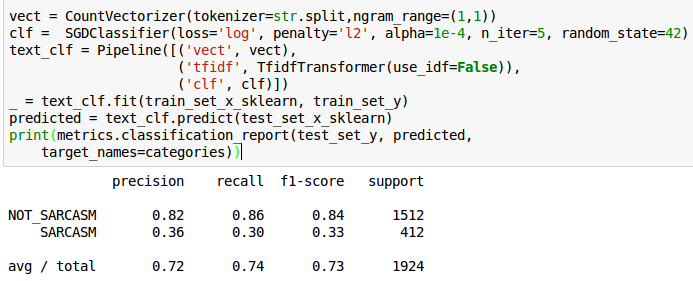
\includegraphics[width=0.5\textwidth]{the-chosen-svm-settings}
\caption{The SVM settings and evaluation set chosen after several trials}
\label{fig:results-choosing-svm-and-data}
\end{figure}

\begin{table}
\centering
\begin{tabular}{ | c | c c c |} 
\hline
Heuristic & Re & Pr & F1 \\
 \hline
 \multicolumn{4}{|c|}{Original Evaluation set} \\
 \hline
 Positive VPs & 0.28 & 0.45 & 0.35 \\ 
 Negative situations & 0.29 & 0.38 & 0.33 \\ 
 (+VPs, –Situations), Unord. & 0.11 & 0.56 & 0.18 \\ 
 (+VPs, –Situations), Ord. & 0.09 & 0.70 & 0.15 \\ 
 \hline
  \multicolumn{4}{|c|}{Our Evaluation (sub)set} \\
  \hline
 Positive VPs & 0.44 & 0.40 & 0.42 \\ 
 Negative situations & 0.31 & 0.37 & 0.33 \\ 
 (+VPs, –Situations), Unord. & 0.20 & 0.46 & 0.28 \\ 
 (+VPs, –Situations), Ord. & 0.12 & 0.60 & 0.21 \\ 
 \hline
\end{tabular}
\caption{A result-based comparison of the original evaluation set with the new evaluation set}
\label{table:1}
\end{table}

\cite{riloff2013sarcasm} used 3000 tweets for evaluation, and 200 separate tweets as a tuning set. Human annotators labeled these tweets as being sarcastic or not sarcastic. We obtained a list of the tweet ids of the 3000 evaluation set tweets, with the corresponding `SARCASM" or `NOT\_SARCASM" label. Not all of these tweets could be recovered, however. We attribute this loss of tweets to either account deletions or privacy setting changes. We recovered 2124 of the tweets, 1666 labeled NOT\_SARCASM and 458 labeled SARCASM. Of these we choose 1924 tweets randomly for our evaluation, while the other 200 are used as a training set.

\begin{table*}
\centering
\begin{tabular}{ | c | c c c | c c c |} 
\hline
  & \multicolumn{3}{|c|}{DatasetSarc} & \multicolumn{3}{|c|}{DatasetYeahright} \\
\hline
Heuristic & Re & Pr & F1 & Re & Pr & F1 \\
 \hline
 \multicolumn{7}{|c|}{Bootstrapping variation A} \\
 \hline
 Positive VPs & 0.21 & 0.47 & 0.29  & 0.05 & 0.44 & 0.10   \\ 
 Negative situations & 0.02 & 0.26 & 0.04  & 0.08 & 0.35 & 0.14 \\ 
 (+VPs, –Situations), Unord. & 0.01 & 0.80 & 0.02  & 0.00 & 1.00 & 0.00 \\ 
 (+VPs, –Situations), Ord. & 0.01 & 0.80 & 0.02 & 0.00 & 0.00 & 0.00  \\ 
 \hline
  \multicolumn{7}{|c|}{Bootstrapping variation B} \\
  \hline
 Positive VPs  & 0.11 & 0.57 & 0.19 & 0.07 & 0.44 & 0.11 \\ 
 Negative situations & 0.19 & 0.40 & 0.26 & 0.11 & 0.35 & 0.17 \\ 
 (+VPs, –Situations), Unord. & 0.03 & 0.75 & 0.06 & 0.00 & 0.25 & 0.00 \\ 
 (+VPs, –Situations), Ord.  & 0.03 & 0.73 & 0.05 & 0.00 & 0.00 & 0.00 \\ 
 \hline
  \multicolumn{7}{|c|}{Bootstrapping variation C} \\
  \hline
 Positive VPs & 0.07 & 0.37 & 0.12 & 0.06 & 0.43 & 0.10 \\ 
 Negative situations & 0.22 & 0.37 & 0.28 & 0.17 & 0.38 & 0.24 \\ 
 (+VPs, –Situations), Unord. & 0.02 & 0.54 & 0.03 & 0.02 & 0.70 & 0.03 \\ 
 (+VPs, –Situations), Ord.  & 0.01 & 0.50 & 0.03 & 0.01 & 0.67 & 0.03 \\ 
 \hline
\end{tabular}
\caption{Experimental results comparing wordlists culled using (a) \#sarcasm (b) \{\#not, \#yeahright, \#justkidding...\} }
\label{table:results}
\end{table*}

\begin{table}
\centering
\begin{tabular}{ | c | c c | c c |} 
\hline
 &  \multicolumn{2}{|c|}{Retrieved} & \multicolumn{2}{|c|}{Discarded} \\
\hline
 & Pos & Neg & Pos & Neg \\
 \hline
 Original paper & 26 & 239 & N/A & N/A \\
 \hline
 \#Sarc Algo A & 2 & 20 & 166 & 731 \\
 \hline
 \#Yeahright Algo A & 11 & 24 & 312 & 495 \\
 \hline
 \#Sarc Algo B & 18 & 46 & 481 & 1239 \\
 \hline
 \#Yeahright Algo B & 18 & 40 & 405 & 1508 \\
 \hline
 \#Sarc Algo C & 19 & 35 & 578 & 336 \\
 \hline
 \#Yeahright Algo C & 17 & 18 & 409 & 269 \\
 \hline
\end{tabular}
\caption{Comparison of the number of words returned by algorithms}
\label{table:num-words-lexicon}
\end{table}

\begin{table}
\centering
\begin{tabular}{ | c | c c | c c |}
\hline
  & 
  \multicolumn{2}{|c|}{\vtop{\hbox{\strut Retrieved}\hbox{\strut intersect}\hbox{\strut Original}\hbox{\strut lexicon}}} & 
  \multicolumn{2}{|c|}{\vtop{\hbox{\strut Discarded}\hbox{\strut intersect}\hbox{\strut Original}\hbox{\strut lexicon}}} \\
\hline
 & Pos & Neg & Pos & Neg \\
 \hline
 \#Sarc Algo A & 1 & 10 & 7 & 78 \\
 \hline
 \#Yeahright Algo A & 0 & 8 & 6 & 59 \\
 \hline
 \#Sarc Algo B & 1 & 22 & 12 & 94 \\
 \hline
 \#Yeahright Algo B & 0 & 10 & 8 & 65 \\
 \hline
 \#Sarc Algo C & 0 & 28 & 14 & 71 \\
 \hline
 \#Yeahright Algo C & 1 & 13 & 10 & 61 \\
 \hline
\end{tabular}
\caption{How many words returned by our algorithms+dataset combination were part of the original work's lexicon?}
\label{table:lexicon-intersect-original}
\end{table}

We noticed that different splits of training and testing sets gave very different results in classification of tweets as sarcastic. We focus on the f1-score of SARCASM labeled tweets for analysis here. For a particular split of data into training and evaluation sets, a precision, recall, f1score triple of \(0.45, 0.41, 0.43\) was observed with an SVM with hinge loss, using TF-IDF with unigrams as features. However, having not saved the data-split, we were unable to produce the same results again with other random splits. After a number of trials, we fixed the split that gave a precision, recall, f1score triple of \(0.36, 0.30, 0.33\). The parameters for the SVM in this case were a log loss SVM, using term frequencies (no IDF) with unigrams as features (Figure \ref{fig:results-choosing-svm-and-data}). All other settings that were tried can be found here: \url{https://goo.gl/eqvEvu}. To summarize, the evaluation set used contains 412 tweets labeled as being sarcastic by annotators, and 1512 tweets considered not sarcastic, with 200 tweets being held out for training the SVM.

In the original evaluation set, there were 23\% sarcastic tweets, while in our evaluation set, there are 21\%. Since the experiment isn't an exact reproduction of the original experiment, we thought it necessary to calculate the classification metrics for \cite{riloff2013sarcasm}'s original word list on the new (effectively subsampled) evaluation set. All else remaining equal, we can expect to see a slight improvement in precision with a possible drop in recall. The results are shown in Table \ref{table:1}, and they confirm this hypothesis. We see that the new values of precision and F1-score and slight overestimates of the original values, while new recall values are underestimates of the original.

We now discuss the efficiency of DatasetYeahright and DatasetSarc, comparing the two with each other as well as collecting positive and negative phrases that are indicators of sarcasm. For each of these bootsrapping datasets, we also have three variations in the lexicon building algorithm. Initially they began as bugs/misinterpretations in the algorithm being coded, but then I thought, why not - seems like a legitimate way of collecting phrases. 
\begin{itemize}
\item A:  This contains an interpretation of the algorithm which finds candidate phrases looking at only one opposite polarity phrase at a time. e.g. Get all negative phrases for `love', then all negative phrases for `really like' etc.
\item B: This contains an interpretation which finds candidate phrases looking at the entire opposite polarity set. e.g. Get all negative phrases for {`love',`really like'} etc. 
\item C: This contains an interpretation which correctly understands subsumption. So far e.g. `waiting forever' was chosen over `waiting'. Now, waiting is chosen.  
\end{itemize}

The classifier evaluation was similar to \cite{riloff2013sarcasm}. For the baseline, an SVM classifier using unigrams as features, which had the highest precision (among baselines), was used, courtesy of scikit-learn libraries \cite{scikit-learn}.

We see in Table \ref{table:results} that the results are similar in the context of this experiment, but quite different compared to the original paper. We immediately notice that recall scores on sarcasm indicators are pretty dismal. This is worth immediate investigation. Comparatively, the two datasets look close in results. It seems like DatasetYeahright has better precision than DatasetSarc. But at these levels of recall, I wouldn't read much into the results. Also, a first glance at the outputs - the returned lexicon - point to a significant amount of difference; between the datasets, as well as the original Riloff lexicon.

We begin investigation of the poor recall by the number of terms in the lexicon. We see in Table \ref{table:num-words-lexicon} that there are far fewer terms in the lexicons returned by our algorithm compared to the original work. Whereas \cite{riloff2013sarcasm} had 239 negative situations, we have no more than 40. We hypothesize that there might be three reasons for this: (1) Incorrect code, especially where selection of the terms based on tagger output is concerned (2) The absence of implementation of the Positive predicative terms (3) The threshold and word limit for acceptance of terms is too low. There is support for the third hypothesis in the number of discards seen in Table \ref{table:num-words-lexicon}. Note that when we say discards, we mean that the algorithm did pick up the phrase as matching the required pattern, but then actively did not include it in the final list. The algorithm discards phrases when (a) there are more than 20 phrases that have a probability of 0.8 or greater of occurrence in sarcastic tweets, or (b) there are fewer than 3 occurrences of the phrase in the sarcastic tweets, or (c) the probability of occurrence of the phrase in the sarcastic tweets is less than 0.8 (0.7 for positive phrases).

Table \ref{table:lexicon-intersect-original} does shows how there are a number of discards that should rather have been in the retrieved column. Another look at Table \ref{table:lexicon-intersect-original} leaves a lot to be desired. We notice that only one, sometimes none, of the positive words in the original lexicon have been recovered. Out of curiosity I checked to see what the words were: `love', `excited', and `just keeps' respectively. However, to look on the brighter side, this is a good proxy to measure how well our algorithm is doing, at least in terms of recovering words in the original lexicon. 

\begin{figure}
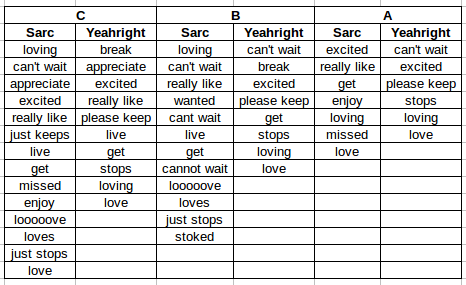
\includegraphics[width=0.5\textwidth]{discarded-terms-in-original-work}
\caption{Positive phrases from the original that were discarded by our algorithm}
\label{fig:discarded-terms-in-original-work}
\end{figure}

Figure \ref{fig:discarded-terms-in-original-work} shows what terms in the original work were discarded by our algorithm. This is one key to understanding the low recall. Note that important words, including the seed - love - were discarded. We will immediately look into why this might be the case and issue a fix.

%6.	Will you build a functioning system?
%7.	What existing tools, if any, do you hope to leverage?
\section{System and tools}

CMU’s part-of-speech tagger designed for tweets (Owoputi et al., 2013), and scikit-learn \cite{scikit-learn} for SVM were used.

\section{Future work}

So far we have separated the \#sarcasm marked tweets from the the other sarcasm marking hashtags that we are exploring. One obvious strategy would be to combine the two tweet datasets and see how well the lexicon returned by this dataset performs.

\section{References}
\bibliography{acl2016}
\bibliographystyle{acl2016}

\end{document}
